% IEEE conference paper source. Compile with: tectonic -X compile main.tex
\documentclass[conference]{IEEEtran}
\usepackage[T1]{fontenc}
\usepackage{microtype}
\usepackage{graphicx}
\usepackage{booktabs}
\usepackage{balance}
\usepackage{multirow}
\usepackage{xcolor}
\usepackage{amsmath,amssymb}
\usepackage{tikz}
\usetikzlibrary{arrows.meta,positioning,shapes.geometric}
\usepackage[hidelinks]{hyperref}
\newcommand{\best}[1]{\textbf{#1}}
\newcommand{\dataset}{KIIT-MiTA}
\newcommand{\battlenet}{BattleNet}
\title{BattleNet: A Resource-Conscious Multi-Label Vision Pipeline for\
Military Object Recognition in Miniature-Art Imagery}
\author{\IEEEauthorblockN{Anonymous Author(s)}
\IEEEauthorblockA{Author details withheld for review\\
Bangladesh}}
\begin{document}
\maketitle

\begin{abstract}
Images used in visual training and archival collections often contain more than one relevant object, yet small, stylized collections make reliable multi-label recognition difficult. This paper studies seven military-object labels in miniature-art imagery using the KIIT-MiTA benchmark. We introduce BattleNet, a task-specific prediction head placed on an ImageNet-initialized hierarchical transformer backbone. The head combines feature projection, squeeze-and-excitation channel recalibration, a residual multilayer perceptron, and a learnable label co-occurrence layer; training uses a sigmoid binary cross-entropy objective and a two-stage transfer-learning schedule. On the held-out 170-image test partition, BattleNet obtains 0.8178 micro-F1, 0.8319 macro-F1, and 0.6706 exact-match accuracy. It exceeds each retained CNN and EfficientNet baseline in micro-F1 and gives strong radar, artillery, and rocket-launcher recognition. For Bangladesh, the result is relevant to image indexing in classrooms and archival collections, but it does not establish performance on local data or operational imagery.
\end{abstract}

\begin{IEEEkeywords}
multi-label classification, hierarchical vision transformer, transfer learning, miniature art, Bangladesh, responsible AI
\end{IEEEkeywords}

\section{Introduction}
Visual collections used for educational interpretation and historical archiving rarely present a single, clean object. A miniature-art scene may contain personnel, vehicles, artillery, and radar-like structures together, often at small scale and with stylized texture. The task is consequently multi-label classification: given one image, identify every present category rather than force the scene into one class. This preserves co-occurring content that a single-label classifier would discard.

In Bangladesh, a classifier of this kind is relevant to image indexing, classroom discussion, and preparation of archival material. It is not a surveillance, targeting, or operational decision system. The data evaluated here are not Bangladesh-specific; the application discussion identifies a possible archival use, not local field validity.

Pretrained visual backbones are attractive in small-data settings because they transfer broad visual representations learned from ImageNet \cite{russakovsky2015imagenet}. Hierarchical visual transformers make it possible to combine local detail with broader scene context. However, a standard linear classifier does not explicitly express channel relevance or label co-occurrence. We therefore design BattleNet to refine the pretrained representation for a small, multi-label collection.

Our contributions are threefold. First, we define a seven-class multi-label setting for \dataset{} with a two-stage fine-tuning procedure and thresholded evaluation. Second, we introduce \battlenet{}, a transformer-based model with channel recalibration, residual transformation, and label co-occurrence modeling. Third, we report held-out performance, class-level error patterns, and the effect of stronger augmentation.

\section{Related Work and Problem Setting}
Convolutional backbones such as ResNet \cite{he2016resnet} and EfficientNet \cite{tan2019efficientnet} have provided strong image-recognition baselines, while vision transformers apply self-attention to image representations \cite{dosovitskiy2021vit}. Hierarchical transformer features retain local visual structure while building larger-context representations, which is valuable for small, stylized scenes. We use an ImageNet-initialized transformer feature extractor rather than train one from scratch on a small collection.

Channel recalibration is motivated by squeeze-and-excitation (SE) networks, which model interdependencies among feature channels \cite{hu2018senet}. BattleNet applies this idea after transformer feature extraction, then adds a residual MLP and a learnable class-to-class correction. These components focus learning on category-specific evidence in a limited-data setting.

Let $\mathcal{D}=\{(x_n,y_n)\}_{n=1}^{N}$, where $x_n$ is an RGB image and $y_n\in\{0,1\}^{C}$ is a multi-hot label vector for $C=7$ classes: artillery, missile, radar, multiple rocket launcher, soldier, tank, and vehicle. The model produces logits $z=f_\theta(x)\in\mathbb{R}^{C}$ and independent probabilities $p_c=\sigma(z_c)$. At evaluation, label $c$ is predicted when $p_c\geq0.5$. Exact-match accuracy requires every label in the vector to be correct; micro-F1 aggregates decisions across all images and labels, whereas macro-F1 gives each class equal weight.
This formulation follows the standard multi-label learning setting in which an instance may belong to several non-exclusive classes \cite{tsoumakas2010multilabel}.

\section{Method}
\subsection{BattleNet architecture}
Figure \ref{fig:architecture} shows the complete forward path. An ImageNet-initialized transformer maps a $224\times224$ image to a 768-dimensional feature vector $h$. BattleNet first projects this representation, applies layer normalization \cite{ba2016layer}, GELU activation \cite{hendrycks2016gelu}, and dropout ($0.3$) \cite{srivastava2014dropout}. An SE block recalibrates channels, followed by batch normalization \cite{ioffe2015batch}; its output is added residually to the projected features. A second residual MLP block adds nonlinear transformation without discarding the original representation. Finally, a linear classifier produces seven logits and a learnable $7\times7$ label-co-occurrence transform adjusts them before the sigmoid output. The reported evaluation uses the primary logits only; no auxiliary-loss result is reported.

\begin{figure*}[!t]
\centering
\resizebox{\textwidth}{!}{%
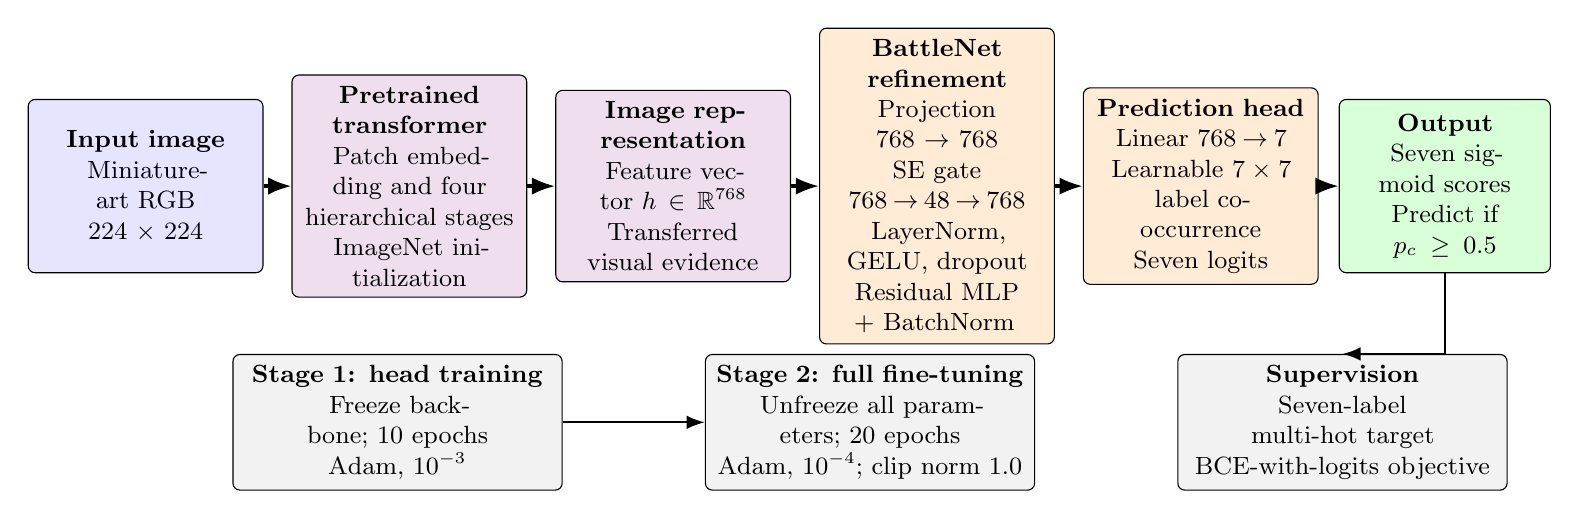
\begin{tikzpicture}[font=\small, >=Latex,
box/.style={draw, rounded corners=2.5pt, align=center, minimum height=22mm, text width=27mm, inner sep=4pt},
input/.style={box, fill=blue!10}, backbone/.style={box, fill=violet!13}, head/.style={box, fill=orange!16}, output/.style={box, fill=green!15}, train/.style={draw, rounded corners=2.5pt, align=center, fill=gray!10, minimum height=14mm, text width=39mm, inner sep=4pt}]
\node[input] (in) at (0,1.6) {\textbf{Input image}\\Miniature-art RGB\\$224\times224$};
\node[backbone] (backbone) at (3.35,1.6) {\textbf{Pretrained transformer}\\Patch embedding and four hierarchical stages\\ImageNet initialization};
\node[backbone] (feat) at (6.70,1.6) {\textbf{Image representation}\\Feature vector $h\in\mathbb{R}^{768}$\\Transferred visual evidence};
\node[head] (refine) at (10.05,1.6) {\textbf{BattleNet refinement}\\Projection $768\!\rightarrow\!768$\\SE gate $768\!\rightarrow\!48\!\rightarrow\!768$\\LayerNorm, GELU, dropout\\Residual MLP + BatchNorm};
\node[head] (label) at (13.40,1.6) {\textbf{Prediction head}\\Linear $768\!\rightarrow\!7$\\Learnable $7\times7$\\label co-occurrence\\Seven logits};
\node[output, text width=24mm] (out) at (16.50,1.6) {\textbf{Output}\\Seven sigmoid scores\\Predict if $p_c\geq0.5$};
\draw[->, very thick] (in) -- (backbone); \draw[->, very thick] (backbone) -- (feat); \draw[->, very thick] (feat) -- (refine); \draw[->, very thick] (refine) -- (label); \draw[->, very thick] (label) -- (out);
\node[train] (stage1) at (3.2,-1.4) {\textbf{Stage 1: head training}\\Freeze backbone; 10 epochs\\Adam, $10^{-3}$};
\node[train] (stage2) at (9.2,-1.4) {\textbf{Stage 2: full fine-tuning}\\Unfreeze all parameters; 20 epochs\\Adam, $10^{-4}$; clip norm 1.0};
\node[train] (loss) at (15.2,-1.4) {\textbf{Supervision}\\Seven-label multi-hot target\\BCE-with-logits objective};
\draw[->, thick] (stage1) -- (stage2); \draw[->, thick] (out.south) |- (loss.north);
\end{tikzpicture}}
\caption{BattleNet methodology and training schedule. The upper path is a single left-to-right inference route, from image to seven sigmoid scores. The lower path independently records the two-stage optimization and BCE-with-logits supervision used for the selected run.}
\label{fig:architecture}
\end{figure*}

\subsection{Objective and optimization}
For a mini-batch of $B$ images, the binary cross-entropy with logits objective is
\begin{equation}
\mathcal{L}(\theta)=-\frac{1}{BC}\sum_{n=1}^{B}\sum_{c=1}^{C}\left[y_{nc}\log p_{nc}+(1-y_{nc})\log(1-p_{nc})\right].
\label{eq:bce}
\end{equation}
The sigmoid derivative yields $\partial\mathcal{L}/\partial z_{nc}=(p_{nc}-y_{nc})/(BC)$, which backpropagation carries through the classifier, head, and backbone. Parameters are updated with Adam \cite{kingma2015adam}; its moving first and second gradient moments give adaptive coordinate-wise steps. Gradients are clipped to norm 1.0 in the implementation, a safeguard against unstable updates during fine-tuning.

Training proceeds in two stages. The backbone is frozen for ten epochs while the head learns at $10^{-3}$, then the complete model is fine-tuned for twenty epochs at $10^{-4}$. This schedule limits destructive early updates to pretrained features. Regularization comes from dropout, weight decay ($10^{-3}$ in the selected experiment), and baseline geometric augmentation: random crop at scale 0.8--1.0, horizontal flip with probability 0.5, and rotation within $\pm15^\circ$. Such transformations are commonly used to improve data diversity, but their validity remains task dependent \cite{shorten2019augmentation}. Stronger augmentation was also run, but it produced 0.7846 micro-F1 for BattleNet versus 0.8178 for the selected baseline-augmentation run; on this small benchmark, stronger perturbations did not help.

\section{Experimental Protocol}
\subsection{Data and implementation}
The local \dataset{} archive contains 1,700 images: 1,360 training, 170 validation, and 170 test examples, with an average of 1.27, 1.24, and 1.28 labels per image, respectively. Images are resized to $224\times224$ and normalized with ImageNet mean and standard deviation. All reported models use the same split and a 0.5 decision threshold. We selected the best recorded test run for each architecture in the project results directory; this selection is a limitation because repeated-seed estimates are not available.

\subsection{Evaluation protocol}
The test partition is held out from training, and all three metrics are computed after thresholding each of the seven sigmoid outputs at 0.5. Micro-F1 counts label decisions jointly, macro-F1 gives the seven labels equal weight, and exact match requires the full predicted label set to agree with the ground truth. Reporting the three together matters here: a model can improve frequent or visually easy labels while still failing to recover every object in a crowded scene. The class table and Figure \ref{fig:battlenet-analysis} therefore accompany the aggregate score rather than treating micro-F1 as a complete account of performance.

Each reported value comes from one recorded run under the image resolution, training schedule, optimizer, regularization, and threshold stated in Section III. Repeated-seed estimates are unavailable, so the reported differences are observations rather than significance claims. The comparison is limited to the retained baselines in Table \ref{tab:main-results}; elapsed time is not used for ranking because experiments were run on different hardware.

The retained comparison contains common CNNs, a ViT, an EfficientNetV2 model, and BattleNet. We report micro-F1, macro-F1, and exact-match accuracy because a single accuracy number can conceal label imbalance and partially correct multi-label predictions. The training records show experiments on CUDA and Apple MPS devices; hardware is not held constant, so elapsed time is not used as a model-ranking metric.

Figure \ref{fig:battlenet-analysis} consolidates the proposed-model analysis: held-out class scores, the underlying correct and incorrect decisions, the retained baseline comparison, and the recorded augmentation contrast. It complements, rather than replaces, the tabulated held-out metrics.

\section{Results and Discussion}
Table \ref{tab:main-results} provides the principal comparison. BattleNet achieves the highest micro-F1 and macro-F1 among the retained baselines, improving on the best EfficientNetV2-S run by 0.0094 micro-F1. Its exact-match accuracy equals the best retained EfficientNetV2-S result while providing a stronger macro-F1, which suggests balanced recognition across the seven classes.

\begin{table}[t]
\caption{Held-out test results for the proposed model and retained baselines. Higher is better.}
\label{tab:main-results}
\centering
\footnotesize
\begin{tabular}{lccc}
\toprule
Model & Micro-F1 $\uparrow$ & Macro-F1 $\uparrow$ & Exact $\uparrow$\\
\midrule
VGG16 & 0.7021 & 0.7143 & 0.5118\\
MobileNetV2 & 0.7286 & 0.7385 & 0.5588\\
ResNet-50 & 0.7598 & 0.7725 & 0.6118\\
ViT-B/16 & 0.7563 & 0.7747 & 0.5882\\
EfficientNetV2-S & 0.8084 & 0.8234 & 0.6706\\
\best{BattleNet (proposed)} & \best{0.8178} & \best{0.8319} & \best{0.6706}\\
\bottomrule
\end{tabular}
\end{table}

Class-wise results for the selected BattleNet run identify the practical weak points. Radar achieves 0.9434 F1, followed by artillery (0.8947) and multiple rocket launcher (0.8679). Soldier (0.7536) and vehicle (0.7527) are the lowest categories. These categories are visually broad and have more opportunities for contextual overlap in dense scenes; this is an interpretation, not a causal proof. The small test set also means that a few image-level mistakes can noticeably move a class metric. For example, the vehicle class has 11 false positives and 12 false negatives among 170 test images.

\begin{table}[t]
\caption{Selected BattleNet run: held-out per-class metrics. Higher is better.}
\label{tab:class-results}
\centering
\footnotesize
\begin{tabular}{lccc}
\toprule
Class & Precision $\uparrow$ & Recall $\uparrow$ & F1 $\uparrow$\\
\midrule
Artillery & 0.8947 & 0.8947 & 0.8947\\
Missile & 0.8333 & 0.8000 & 0.8163\\
Radar & 0.9615 & 0.9259 & \best{0.9434}\\
Rocket launcher & 0.9200 & 0.8214 & 0.8679\\
Soldier & 0.7647 & 0.7429 & 0.7536\\
Tank & 0.8056 & 0.7838 & 0.7945\\
Vehicle & 0.7609 & 0.7447 & 0.7527\\
\bottomrule
\end{tabular}
\end{table}

\begin{figure*}[!t]
\centering
\resizebox{0.96\textwidth}{!}{%
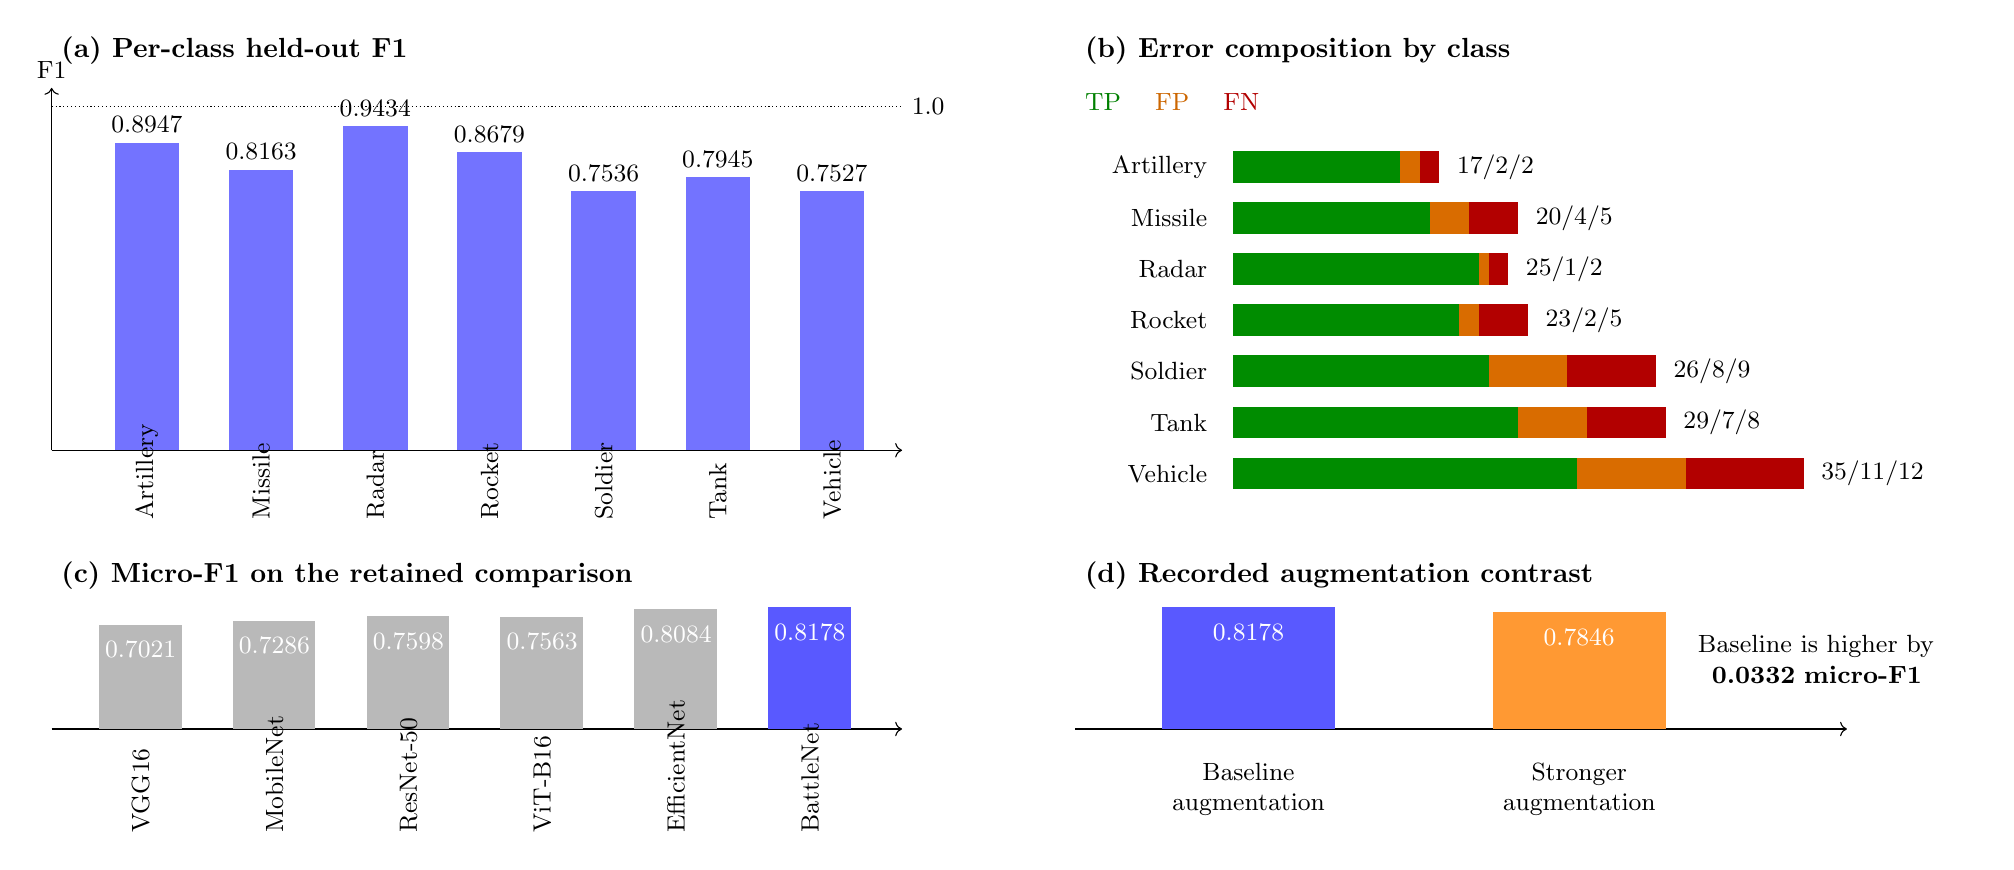
\begin{tikzpicture}[font=\small, yscale=1.18]
\node[anchor=west, font=\bfseries] at (0,7.3) {(a) Per-class held-out F1};
\draw[->] (0,3.0) -- (0,6.9) node[above] {F1};
\draw[->] (0,3.0) -- (10.8,3.0);
\foreach \x/\n/\v in {0.8/Artillery/0.8947,2.25/Missile/0.8163,3.70/Radar/0.9434,5.15/Rocket/0.8679,6.60/Soldier/0.7536,8.05/Tank/0.7945,9.50/Vehicle/0.7527} {
  \pgfmathsetmacro\h{3.7*\v}
  \fill[blue!55] (\x,3.0) rectangle +(0.82,\h);
  \node[rotate=90, anchor=west] at (\x+0.41,2.15) {\n};
  \node[anchor=south] at (\x+0.41,3.0+\h) {\v}; }
\draw[densely dotted] (0,6.7) -- (10.8,6.7) node[right] {1.0};

\node[anchor=west, font=\bfseries] at (13.0,7.3) {(b) Error composition by class};
\node[anchor=west] at (13.0,6.75) {\textcolor{green!50!black}{TP} \quad \textcolor{orange!80!black}{FP} \quad \textcolor{red!70!black}{FN}};
\foreach \y/\n/\tp/\fp/\fn in {6.05/Artillery/17/2/2,5.50/Missile/20/4/5,4.95/Radar/25/1/2,4.40/Rocket/23/2/5,3.85/Soldier/26/8/9,3.30/Tank/29/7/8,2.75/Vehicle/35/11/12} {
  \node[anchor=east] at (14.8,\y) {\n};
  \fill[green!55!black] (15.0,{\y-0.17}) rectangle +({\tp/8},0.34);
  \fill[orange!85!black] ({15.0+\tp/8},{\y-0.17}) rectangle +({\fp/8},0.34);
  \fill[red!70!black] ({15.0+(\tp+\fp)/8},{\y-0.17}) rectangle +({\fn/8},0.34);
  \node[anchor=west] at ({15.1+(\tp+\fp+\fn)/8},\y) {\tp/\fp/\fn}; }

\node[anchor=west, font=\bfseries] at (0,1.65) {(c) Micro-F1 on the retained comparison};
\draw[->] (0,0) -- (10.8,0);
\foreach \x/\n/\v/\c in {0.6/VGG16/0.7021/gray!55,2.3/MobileNet/0.7286/gray!55,4.0/ResNet-50/0.7598/gray!55,5.7/ViT-B16/0.7563/gray!55,7.4/EfficientNet/0.8084/gray!55,9.1/BattleNet/0.8178/blue!65} {
  \pgfmathsetmacro\h{1.6*\v}
  \fill[\c] (\x,0) rectangle +(1.05,\h);
  \node[rotate=90, anchor=west] at (\x+0.53,-1.22) {\n};
  \node[anchor=north, text=white] at (\x+0.53,{\h-0.08}) {\v}; }

\node[anchor=west, font=\bfseries] at (13.0,1.65) {(d) Recorded augmentation contrast};
\draw[->] (13.0,0) -- (22.8,0);
\fill[blue!65] (14.1,0) rectangle +(2.2,1.309); \node[anchor=north, text=white] at (15.2,1.23) {0.8178};
\fill[orange!80] (18.3,0) rectangle +(2.2,1.255); \node[anchor=north, text=white] at (19.4,1.18) {0.7846};
\node[align=center] at (15.2,-0.65) {Baseline\\augmentation};
\node[align=center] at (19.4,-0.65) {Stronger\\augmentation};
\node[align=center, text width=41mm] at (22.4,0.75) {Baseline is higher by\\\textbf{0.0332 micro-F1}};
\end{tikzpicture}}
\caption{BattleNet-only analysis from the selected 170-image held-out test run. (a) F1 varies materially by label; (b) reports the corresponding true-positive, false-positive, and false-negative counts; (c) compares only the baselines reported in Table \ref{tab:main-results}; and (d) shows the two recorded augmentation configurations. Bars in (c) and (d) are single recorded runs, not confidence intervals.}
\label{fig:battlenet-analysis}
\end{figure*}

Figure \ref{fig:battlenet-analysis}(a)--(b) makes the class-level trade-offs visible. Radar is the most reliable category, with 25 true positives against one false positive and two false negatives. Vehicle is a clear review priority: it has the lowest F1 and the largest error total (11 false positives and 12 false negatives). Soldier shows a similar pattern, with 17 errors. These counts support targeting future annotation review and threshold analysis at broad, context-dependent categories rather than treating the aggregate micro-F1 as uniformly representative.

The comparative panels also bound the result appropriately. In Figure \ref{fig:battlenet-analysis}(c), BattleNet improves on the best retained comparator, EfficientNetV2-S, by 0.0094 micro-F1; Table \ref{tab:main-results} provides the associated macro-F1 and exact-match values. Figure \ref{fig:battlenet-analysis}(d) shows that baseline augmentation plus dropout and weight decay outperformed the recorded stronger augmentation by 0.0332 micro-F1. Strong rotations, vertical flips, and more aggressive crops may disrupt visual cues in stylized artwork, but this is one configuration comparison, not a universal augmentation rule. Repeated seeds, calibrated thresholds, and controlled component ablations are necessary before drawing causal conclusions.

The architecture uses LayerNorm, residual paths, pretrained initialization, Adam, and gradient clipping, which are standard mechanisms for maintaining stable signal propagation. This paper does not use a training-loss plot as evidence of generalization: held-out performance, error counts, and the bounded comparisons above are the basis for its analysis. A future study should log gradient norms per stage and compare each head component through controlled ablations.

\subsection{Error analysis}
The error counts identify the difficult classes. Radar has the strongest F1 and only three total errors, whereas vehicle accumulates 23 errors and soldier accumulates 17. Vehicle and soldier labels therefore deserve closer inspection when the model is used to index a collection. The result does not support treating every suggested tag as equally reliable.

False positives and false negatives imply different correction tasks. A false positive adds a tag that a reviewer must remove; a false negative leaves an object untagged unless the reviewer notices it. The vehicle results contain both types in comparable quantity, so simply raising or lowering the common 0.5 threshold is unlikely to solve every error. A subsequent study should inspect class-specific precision--recall curves on validation data, select thresholds without touching the test partition, and report whether a threshold change improves the archival review burden rather than only micro-F1.

The present evidence also cannot isolate why the proposed head improves the retained comparison. Channel recalibration, residual transformation, and label co-occurrence are introduced together, so the 0.0094 micro-F1 margin over EfficientNetV2-S should be read as a system-level observation. The next experimental increment is therefore clear: remove one component at a time under the same split, augment those ablations with repeated seeds, and publish the per-class deltas. Such a design would reveal whether the overall gain is stable and whether it is concentrated in the broad classes that currently require the most human attention.

\subsection{Bangladesh-facing use and safeguards}
For Bangladesh, the relevant near-term use is visual indexing for archival and educational collections, not autonomous recognition. Curators or instructors may use candidate tags while examining scanned or born-digital images and retain the image beside each accepted tag. Any local collection would need Bangla labels and annotation rules that match its own visual material.

This pathway has clear limits. The present labels and imagery do not validate performance on Bangladesh collections, aerial imagery, live video, or any operational context. It must not be used to identify people, guide force, or make high-consequence decisions. Before any local deployment, a Bangladesh-specific data governance process, consent and provenance review, localized annotation guidelines, independent testing, and a human appeal/correction process would be necessary.

In an archival setting, each item should retain its collection identifier, source or rights note, digitization date when known, original image, proposed tags, and reviewer decisions. These fields distinguish a mislabeled image from an ambiguous one and make later corrections traceable. They also keep a confidence score tied to the image and the evidence on which it was assessed.

\section{Conclusion}
This paper examined multi-label recognition of seven military-object categories in miniature-art imagery. BattleNet combines an ImageNet-initialized transformer with feature projection, squeeze-and-excitation recalibration, a residual MLP, and a label co-occurrence transform. On the held-out KIIT-MiTA test set, it reached 0.8178 micro-F1, 0.8319 macro-F1, and 0.6706 exact-match accuracy. Within the retained comparison, BattleNet exceeded EfficientNetV2-S by 0.0094 micro-F1 and matched its exact-match score.

The class results add an important qualification to the aggregate score. Radar, artillery, and rocket launcher were recognized strongly, whereas soldier and vehicle remained difficult. Vehicle alone produced 11 false positives and 12 false negatives. The augmentation comparison also showed that stronger geometric transformations reduced micro-F1 by 0.0332 in the recorded setting. These findings indicate that the current gain is concentrated in a bounded benchmark setting rather than evidence of uniform performance across labels or image conditions.

The comparative margin should also be read with care. BattleNet improved micro-F1 and macro-F1 over the retained baselines, but the improvement over EfficientNetV2-S is small in absolute terms and no component ablation is available. The result therefore supports the combined model as evaluated, not a separate causal claim for channel recalibration, residual transformation, or label co-occurrence. The per-class table is equally important: it shows that a good aggregate score can coexist with weak outcomes in visually broad categories. For indexing work, these categories are where the output warrants the closest inspection.

The two-stage schedule and baseline augmentation were selected from the recorded experiments because they produced the reported test result. Stronger rotation, cropping, and flipping did not improve BattleNet on this collection. In stylized miniature-art scenes, these transformations may alter the spatial cues that distinguish personnel from vehicles or separate a launcher from surrounding equipment. That explanation remains tentative, but the observed drop is sufficient to rule out a simple claim that stronger augmentation is beneficial for this benchmark.

The present study is limited to one stylized collection, one recorded run per reported configuration, and a fixed decision threshold. It does not establish performance on Bangladeshi collections, aerial images, live video, or operational material. The most useful extension is a class-wise study on locally curated archival images: it should test threshold selection, isolate the contribution of each BattleNet component, and examine whether the vehicle and soldier errors persist under local annotation practice. Until then, the model is best understood as a source of candidate index terms for educational and archival material.

\bibliographystyle{IEEEtran}
\balance
\bibliography{references}
\end{document}
